\chapter{Etat de l'art}
\authors{
  \authorinfo{Marc}{de la Motte Rouge} \\
}

Pour d�buter notre projet sur la r�alisation du cockpit, nous avons recherch� des informations sur chaque partie � r�aliser. Pour cela, nous avons organis� des groupes de travail au sein de l��quipe, chaque groupe �tant responsable d�un bloc.

Nous avons d�coup� la r�alisation technique du projet en quatre grandes parties :
- T�che 1 : Saisie des donn�es, commande (vitesse, cap etc �)
- T�che 2 : Commande de pilotage, puissance  (cette partie comprend l�asservissement des commandes)
- T�che 3 : Monde ext�rieur et r�seaux
- T�che 4 : Interface Homme Machine (IHM) et extraction des donn�es de Flight Simulator (FS).
- T�che 5 : Recherche g�n�rale sur le projet, information sur les projets de ce type d�j� r�alis�s.

Ces t�ches sont r�partis de la mani�re suivante dans le cockpit.

\begin{figure}[htpb]
  \centering
  \fbox{
    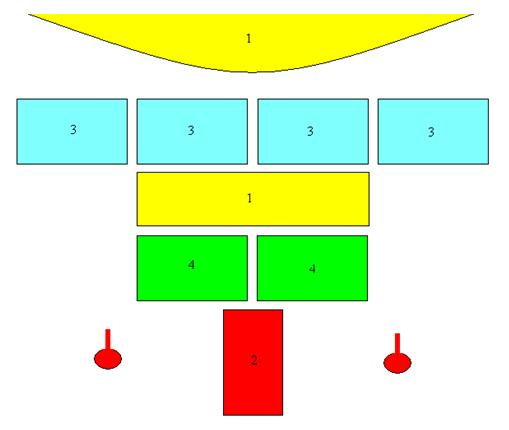
\includegraphics[scale=0.5]{images/decoupage1}
  }
  \caption{D�coupage des parties en d�but de projet}
 % \label{fig:archi_fsadapter}
\end{figure}

Ce d�coupage fut choisi selon le type d'instrument � r�aliser. En effet, les �crans ont fait l'objet d'une partie.